%% LaTeX2e class for student theses
%% sections/content.tex
%% 
%% Karlsruhe Institute of Technology
%% Institute for Program Structures and Data Organization
%% Chair for Software Design and Quality (SDQ)
%%
%% Dr.-Ing. Erik Burger
%% burger@kit.edu
%%
%% Version 1.3.3, 2018-04-17

% TODO find a better title for this chapter
\chapter{Applying RDF2Graph to Wikidata}
\label{ch:RDF2Graph+Wikidata}

% TODO find a better title for this section
\section{General RDF2Graph Updates}
\label{sec:RDF2Graph+Wikidata:updates}

% TODO find a better title for this section
\section{Wikidata Support}
\label{sec:RDF2Graph+Wikidata:Wikidata}

The most fundamental change to make RDF2Graph support Wikidata
was % TODO is?
to change the type predicates used.
RDF2Graph heavily relies on the type information of the RDF graph it inspects,
assuming a one-to-one mapping between classes and shapes,
and it uses the standard predicates \PName{rdf:type} and \PName{rdfs:subClassOf}
to determine the class of a subject and the superclasses of a class, respectively.
However, Wikidata does not use these standard predicates:
the class(es) and superclass(es) of an item
are regular statements like any other Wikidata statement,
using the properties \PL{P31}{instance of} and \PL{P279}{subclass of}.
In the \gls{rdf} export, \PName{rdf:type} and \PName{rdfs:subClassOf} are only used
as part of the meta-model, % TODO meta-model? hm
assigning each item the class \PName{wikibase:Item}, a subclass of \PName{wikibase:Entity}.
To use the type information within the data instead of this meta-model,
RDF2Graph was changed to use the predicates \PName{wdt:P31} and \PName{wdt:P279} % TODO we haven’t seen the wdt: syntax yet, should that be in the Background?
instead of \PName{rdf:type} and \PName{rdfs:subClassOf}.

Another important aspect is that it’s not feasible to run RDF2Graph on the entirety of Wikidata at once.
For example, the 2018-08-20 full Wikidata dump is \SI{42.7}{\giga\byte} large after gzip compression % TODO >300GB uncompressed (309657344438 bytes), which is probably more impressive
and \num{8316156305} lines long uncompressed,
with most lines corresponding to one triple (except for some blank lines).
More importantly, inferring a single schema from all of Wikidata is also not the intention of this work:
the intention is to infer a schema from a particular set of exemplary items, % TODO awkward passive voice (“*the* intention” is *my* intention, I guess)
and ignore similar items which are not as exemplary (e.~g. not as well maintained)
as well as unrelated items. % TODO that should be explained in more detail in the Introduction, which I haven’t written yet as of this writing
So instead of running RDR2Graph directly against the SPARQL endpoint of the Wikidata Query Service,
a process was set up % TODO super awkward passive voice
to download the data of all selected items as well as the items they directly link to,
load that into a single N-Triples file,
serve that file via a local Fuseki SPARQL server,
run RDF2Graph against that server,
and finally run the ShEx exporter against RDF2Graph’s results.
To make it easier to run, the entire process is controlled by a Makefile in the RDF2Graph repository,
so that after creating a \filename{\variable{example}.entities.sparql} file with a SPARQL query selecting the exemplary items,
it is sufficient to run \command{make \variable{example}.shex} to run the entire process and generate the ShEx file.

This data download step also presents a convenient opportunity to drop some data from the items.
For one, the labels, descriptions and aliases of an item can make up a large portion of its data,
but are generally not interesting for ShEx schemas,
since there is rarely more to say about them than
“an item has one or more labels, zero or more descriptions, and zero or more aliases”. % TODO express as ShExC?
% TODO in theory it’s possible for items to have zero labels…
(A manually curated schema might go beyond this –
perhaps requiring, for example, that items about Spanish municipalities have a label in Spanish –
but such details are beyond the ability of RDF2Graph to infer.)
Additionally, Wikidata items often have a number of statements listing external identifiers for the item
(that is, identifiers in other databases for the same concept described by this item):
for example, Wikidata’s \Q{Q80} corresponds to \loc{no99010609} in the \gls{loc},
\viaf{85312226} in the \gls{viaf},
\imdbName{nm3805083} in the \gls{imdb},
\TwitterAccount{timberners\_lee} on Twitter,
and dozens of other external identifiers. % TODO is a vague “dozens” okay?
All these external identifiers are technically just ordinary statements,
but since they are generally not very interesting compared to other statements,
they are sorted into a separate section when viewing the item on the Wikidata website.
To reduce the runtime of the RDF2Graph inference process,
and to reduce clutter in the inferred schemas,
the labels, descriptions, aliases, and external identifiers of an item
are therefore excluded when downloading the data for a set of exemplary items.

However, one unfortunate consequence of running RDF2Graph against a reduced data set
is that RDF2Graph cannot see the full type hierarchy of the classes involved:
for example, depending on how much data was downloaded,
it may or may not be aware that the classes \QL{Q112099}{island nation} and \QL{Q3624078}{sovereign state}
have a common superclass, \QL{Q7275}{state},
which reduces the available options during the simplification step. % TODO not happy with this phrasing
To mitigate this, RDF2Graph was patched % TODO awkward passive voice
to allow specifying an alternative SPARQL endpoint for all queries that require a full view of the data,
and uses this alternative endpoint for the query to get all parent and child classes of a class.
The Makefile-controlled process mentioned above % TODO awkward phrasing
specifies the Wikidata Query Service SPARQL endpoint for this option,
so that RDF2Graph can learn the full class hierarchy around all relevant items % TODO is “learn” the right word?
even when running against a subset of Wikidata. % TODO “subset of Wikidata”? not quite happy with that phrasing

The simplification process also required some changes to support Wikidata.
Originally, RDF2Graph would merge all classes into their superclass,
almost completely unconditionally,
stopping only at the root class \PName{owl:Thing}.
This was much too aggressive for Wikidata:
not only does Wikidata have a different root class (\QL{Q35120}{entity}),
but it also has a complex hierarchy of abstract classes below that root class,
and merging other classes into those abstract classes
(like \QL{Q151885}{concept}, \QL{Q7184903}{abstract object} or \QL{Q830077}{subject})
would not result in useful schemas.
Therefore, the merging step in the simplification process was adapted % TODO awkward passive voice
to add a number of Wikidata items to the set of classes which other classes should not be merged into
(originally only containing \PName{owl:Thing}),
and to stop looking for common superclasses of two classes after checking five levels in the class hierarchy.
(The limit of five levels is an arbitrary choice
and could also be made configurable if deemed necessary in the future.) % TODO look a bit more into this?
% TODO also disabled step 7.4.4 (dropping predicates that were found in superclasses)
% because the superclass support in the ShEx export changed,
% but that requires explanation of how the ShEx export changed

% TODO find a better title for this section
\section{Schema Reduction}
\label{sec:RDF2Graph+Wikidata:schema-reduction}


% TODO find a better title for this chapter
\chapter{The Wikidata ShEx Inference Tool}
\label{ch:wdsi}

% TODO all of the below probably needs to go in a \section, I’m not sure what the rules on chapter introductions are

Once the schema inference process against Wikidata was more or less settled,
it was time to begin making it available to others. % TODO is “it was time to” appropriate language?
RDF2Graph, its ShEx exporter, and the Makefile-based process around them
require several different programs and programming runtimes to be available,
which it would be unreasonable to expect every interested user to install
(not to mention that the Makefile assumes a Unix-like environment and almost certainly does not work on Windows).
Instead, a common approach in the Wikimedia universe
is to install such a program on Wikimedia Toolforge
and make it available to users via a web interface.

% TODO what tense / mood to use in this section? not sure if subjunctive mood makes sense
In this Wikimedia-hosted tool,
users would enter a SPARQL query selecting the set of exemplary items from which to infer a schema,
and the tool would download the associated data,
run RDF2Graph and the ShEx exporter,
and make the ShExC output available to the user.
The simplest process for that would be
to directly return the ShExC code in the server’s response to the user’s HTTP request,
but that is not possible:
even simple inference jobs % TODO “jobs” okay?
from a single item take at least several minutes,
and more complicated jobs % TODO “jobs” again
over several dozens of items can take multiple hours –
the connection to the user would time out long before that,
and the user might also become impatient and simply close their browser window or tab.

Instead, the inference process runs in the background,
and after submitting the SPARQL query and starting the process,
the user is redirected to a page describing the currently running job.
They can periodically reload the page,
and each time the page is loaded,
the tool checks if the background process is still running.
If the background process has finished in the meantime,
the tool collects the output,
cleans up the temporary files left behind by the process,
and finally makes the output
(primarely the ShExC code, but also debugging outputs)
available to the user.

Since this already more or less requires storing inputs and outputs persistently,
a natural extension of this scheme is to make this job page available to others,
so that not only the original submitter but also other users can inspect a running or completed job.
(The input data is entirely public data from Wikidata,
so there is no reason to restrict the visibility of the outputs.)
This facilitates easy collaboration on schemas between multiple users
and allows even casual visitors to see how the tool operates,
and what kinds of results it produces,
without having to start their own inference process.
To make each result easier to comprehend for others,
users can also submit a title, description, and/or URL for additional information
along with their SPARQL query. % TODO strictly speaking, the title isn’t optional. does that matter?

As the inference process consumes a lot of resources,
it doesn’t run directly on the same system as the web server providing the tool’s front-end.
Instead, it is submitted as a job for the Sun Grid Engine system also offered by the Toolforge environment,
where it will be run on some execution host with sufficient free resources.
To ensure that the system’s resources are not exhausted by this one tool,
the tool only allows at most two jobs to run in parallel,
and prevents users from submitting any more jobs if too many jobs are currently running,
instead asking them to try again later.
Job submission is also restricted to users with a valid Wikidata account,
atuhenticated via OAuth.
The identity of the submitting user is another attribute of a job,
along with its title, description, URL, and SPARQL query,
and can be seen by other users who look at the pending or finished jobs of the tool.

% TODO is this paragraph relevant?
Details of each job,
such as its title, submitting user, and submission time,
are stored in a tool-specific SQL database on the Toolforge database servers.
However, the outputs of a job
(ShExC file, standard output of the process, standard error of the process),
as well as to a lesser degree the SPARQL query forming its input,
are too large to store in a database.
Instead, they are stored directly on the file system.

% TODO find a better title for this section
\section{Toolforge Support}
\label{sec:wdsi:Toolforge}

% TODO find a better title for this section
\section{Abstract Considerations}
\label{sec:wdsi:abstract}

% TODO I suppose the current paragraphs directly below the chapter mostly cover this section,
% needs to be suitably rearranged

% TODO find a better title for this section
\section{Utilities}
\label{sec:wdsi:utilities}

To make the ShEx output more readable,
support for the ShExC syntax was added to the popular Pygments syntax highlighter. % TODO link to pull request?
If the ShEx code for a job % TODO is “a job” okay?
is requested by a browser
or some other kind of client which declares that it can accept HTML
(using HTTP content negotiation),
the tool applies the Pygments syntax highlighter to the code on-the-fly
and sends a complete HTML document containing the prettified code and associated CSS rules.
Clients which do not accept HTML documents receive the plain ShExC code instead.

The HTML document that is sent to browsers
also includes a client-side script,
which searches for Wikidata item IDs in the ShExC code,
fetches the labels of all mentioned item IDs from Wikidata,
and adds them to the document in \lstinline[language=html]{<abbr>} abbreviation elements.
It also hyperlinks each reference of a shape to its definition,
and the definition to the corresponding entity on Wikidata.
This makes it much more convenient to read the schema in the browser:
the user merely has to hover their mouse over a class to see its label instead of the item ID;
clicking on it brings the user to the shape for that class;
and clicking on the ID there brings the user to the Wikidata page for the class,
where they can further explore the related data.

A comparison of the effects of these two features
can be seen in \cref{fig:shexc-syntax-highlighting}.

% TODO revisit layout of this figure when the thesis is close to done,
% perhaps adjust the widths and/or trimming depending on how the figure fits on a page
\begin{figure}[t]
  \begin{subfigure}[t]{0.45\textwidth}
    \centering
    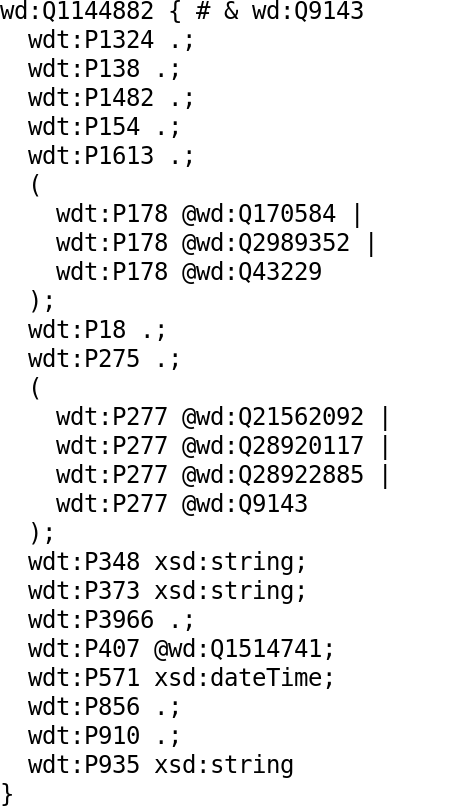
\includegraphics[trim={0 2.5cm 0 0},clip]{screenshots/shexc-no-syntax-highlighting}
    \caption{
      Excerpt of an inferred schema for Linux distributions.
    }
    \label{fig:shexc-syntax-highlighting-without}
  \end{subfigure}
  \begin{subfigure}[t]{0.45\textwidth}
    \centering
    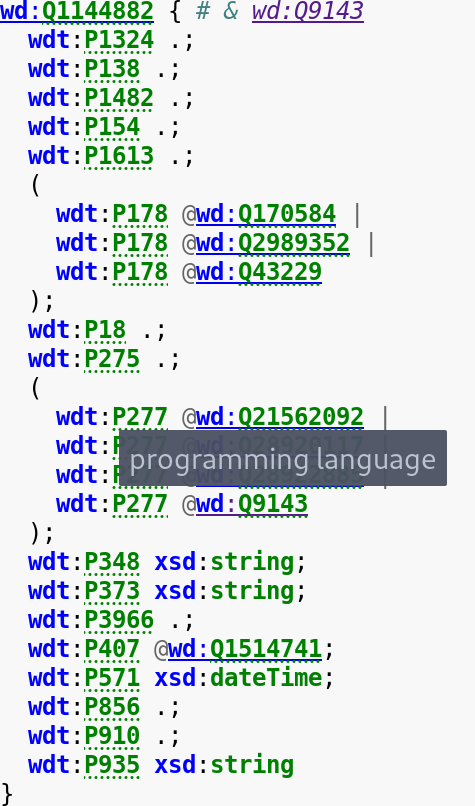
\includegraphics[trim={0 2.5cm 0 0},clip]{screenshots/shexc-with-syntax-highlighting}
    \caption{
      The same schema with syntax highlighting and the script applied.
      The cursor is over the \lstinline{P277} property ID.
    }
    \label{fig:shexc-syntax-highlighting-with}
  \end{subfigure}
  \caption{
    Comparison of the effects of syntax highlighting and the client-side script.
  }
  \label{fig:shexc-syntax-highlighting}
\end{figure}
